\documentclass[10pt,pdf,hyperref={unicode}]{beamer}

\mode<presentation>
{
\usetheme{boxes}
\beamertemplatenavigationsymbolsempty

\setbeamertemplate{footline}[page number]
\setbeamersize{text margin left=1em, text margin right=0.5em}
}

\usepackage[utf8]{inputenc}
\usepackage[english, russian]{babel}
\usepackage[normalem]{ulem}
\usepackage{bm}
\usepackage{multirow}
\usepackage{ragged2e}
\usepackage{indentfirst}
\usepackage{multicol}
\usepackage{subfig}
\usepackage{amsmath,amssymb}
\usepackage{dsfont}
\usepackage{enumerate}
\usepackage{mathtools}
\usepackage{comment}
\usepackage{tabularx, tabulary, multicol}
\usepackage[all]{xy}

\newcommand{\bz}{\mathbf{z}}
\newcommand{\bx}{\mathbf{x}}
\newcommand{\by}{\mathbf{y}}
\newcommand{\bv}{\mathbf{v}}
\newcommand{\bw}{\mathbf{w}}
\newcommand{\ba}{\mathbf{a}}
\newcommand{\bb}{\mathbf{b}}
\newcommand{\bff}{\mathbf{f}}
\newcommand{\bh}{\mathbf{h}}
\newcommand{\bl}{\mathbf{l}}
\newcommand{\bp}{\mathbf{p}}
\newcommand{\bq}{\mathbf{q}}
\newcommand{\bs}{\mathbf{s}}
\newcommand{\bt}{\mathbf{t}}
\newcommand{\bu}{\mathbf{u}}
\newcommand{\bT}{\mathbf{T}}
\newcommand{\bX}{\mathbf{X}}
\newcommand{\bZ}{\mathbf{Z}}
\newcommand{\bS}{\mathbf{S}}
\newcommand{\bH}{\mathbf{H}}
\newcommand{\bW}{\mathbf{W}}
\newcommand{\bY}{\mathbf{Y}}
\newcommand{\bU}{\mathbf{U}}
\newcommand{\bQ}{\mathbf{Q}}
\newcommand{\bP}{\mathbf{P}}
\newcommand{\bA}{\mathbf{A}}
\newcommand{\bB}{\mathbf{B}}
\newcommand{\bC}{\mathbf{C}}
\newcommand{\bE}{\mathbf{E}}
\newcommand{\bF}{\mathbf{F}}
\newcommand{\bsigma}{\boldsymbol{\sigma}}
\newcommand{\bomega}{\boldsymbol{\omega}}
\newcommand{\btheta}{\boldsymbol{\theta}}
\newcommand{\bgamma}{\boldsymbol{\gamma}}
\newcommand{\bdelta}{\boldsymbol{\delta}}
\newcommand{\bPsi}{\boldsymbol{\Psi}}
\newcommand{\bpsi}{\boldsymbol{\psi}}
\newcommand{\bxi}{\boldsymbol{\xi}}
\newcommand{\bmu}{\boldsymbol{\mu}}
\newcommand{\bchi}{\boldsymbol{\chi}}
\newcommand{\bzeta}{\boldsymbol{\zeta}}
\newcommand{\blambda}{\boldsymbol{\lambda}}
\newcommand{\beps}{\boldsymbol{\varepsilon}}
\newcommand{\bZeta}{\boldsymbol{Z}}
% mathcal
\newcommand{\cX}{\mathcal{X}}
\newcommand{\cY}{\mathcal{Y}}
\newcommand{\cW}{\mathcal{W}}

\newcommand{\dH}{\mathds{H}}
\newcommand{\dR}{\mathds{R}}
% transpose
\newcommand{\T}{^{\mathsf{T}}}

% command to strike out text
\newcommand{\stkout}[1]{\ifmmode\text{\sout{\ensuremath{#1}}}\else\sout{#1}\fi}

% limited alertblock
\newenvironment<>{varblock}[2][.9\textwidth]{%
	\setlength{\textwidth}{#1}
	\begin{actionenv}#3%
		\def\insertblocktitle{#2}%
		\par%
		\usebeamertemplate{block begin}}
	{\par%
		\usebeamertemplate{block end}%
	\end{actionenv}}

\renewcommand{\epsilon}{\ensuremath{\varepsilon}}
\renewcommand{\phi}{\ensuremath{\varphi}}
\renewcommand{\kappa}{\ensuremath{\varkappa}}
\renewcommand{\le}{\ensuremath{\leqslant}}
\renewcommand{\leq}{\ensuremath{\leqslant}}
\renewcommand{\ge}{\ensuremath{\geqslant}}
\renewcommand{\geq}{\ensuremath{\geqslant}}
\renewcommand{\emptyset}{\varnothing}

\usepackage{tikz}
\usetikzlibrary{positioning,arrows}

\tikzstyle{name} = [parameters]
\definecolor{name}{rgb}{0.5,0.5,0.5}

\usepackage{caption}
\captionsetup{skip=0pt,belowskip=0pt}

\newtheorem{rustheorem}{Теорема}
\newtheorem{russtatement}{Утверждение}
\newtheorem{rusdefinition}{Определение}

% colors
\definecolor{darkgreen}{rgb}{0.0, 0.2, 0.13}
\definecolor{darkcyan}{rgb}{0.0, 0.55, 0.55}

\AtBeginEnvironment{figure}{\setcounter{subfigure}{0}}

\captionsetup[subfloat]{labelformat=empty}
\addto\captionsrussian{\renewcommand{\figurename}{}}
\graphicspath{{../figures/}}

%----------------------------------------------------------------------------------------------------------

\title[Заголовок]{Выбор моделей пространства состояний в задаче нейронного декодирования}
\author{Владимиров Э.А.}

\institute[]{Московский физико-технический институт}
\date{\footnotesize
	\par\smallskip\emph{Научный руководитель:} д.~ф.-м.~н. В.\,В.~Стрижов
	\par\bigskip\small 2023}

%---------------------------------------------------------------------------------------------------------
\begin{document}

\begin{frame}
\titlepage
\end{frame}

%----------------------------------------------------------------------------------------------------------
\begin{frame}{Модели глубокого обучения в задаче нейронного декодирования}
	\begin{alertblock}{Проблема}
		Моделирование и распознание динамики нейронных систем
	\end{alertblock}
	
	\begin{alertblock}{Задача}
		Выбор модели пространства состояний
	\end{alertblock}
	
	\begin{alertblock}{Решение}
		Сделать выбор на основе анализа свойств моделей
	\end{alertblock}
\end{frame}

%---------------------------------------------------------------------------------------------------------
\begin{frame}{Модель пространства состояний (SSM)}
	\begin{multicols}{2}
		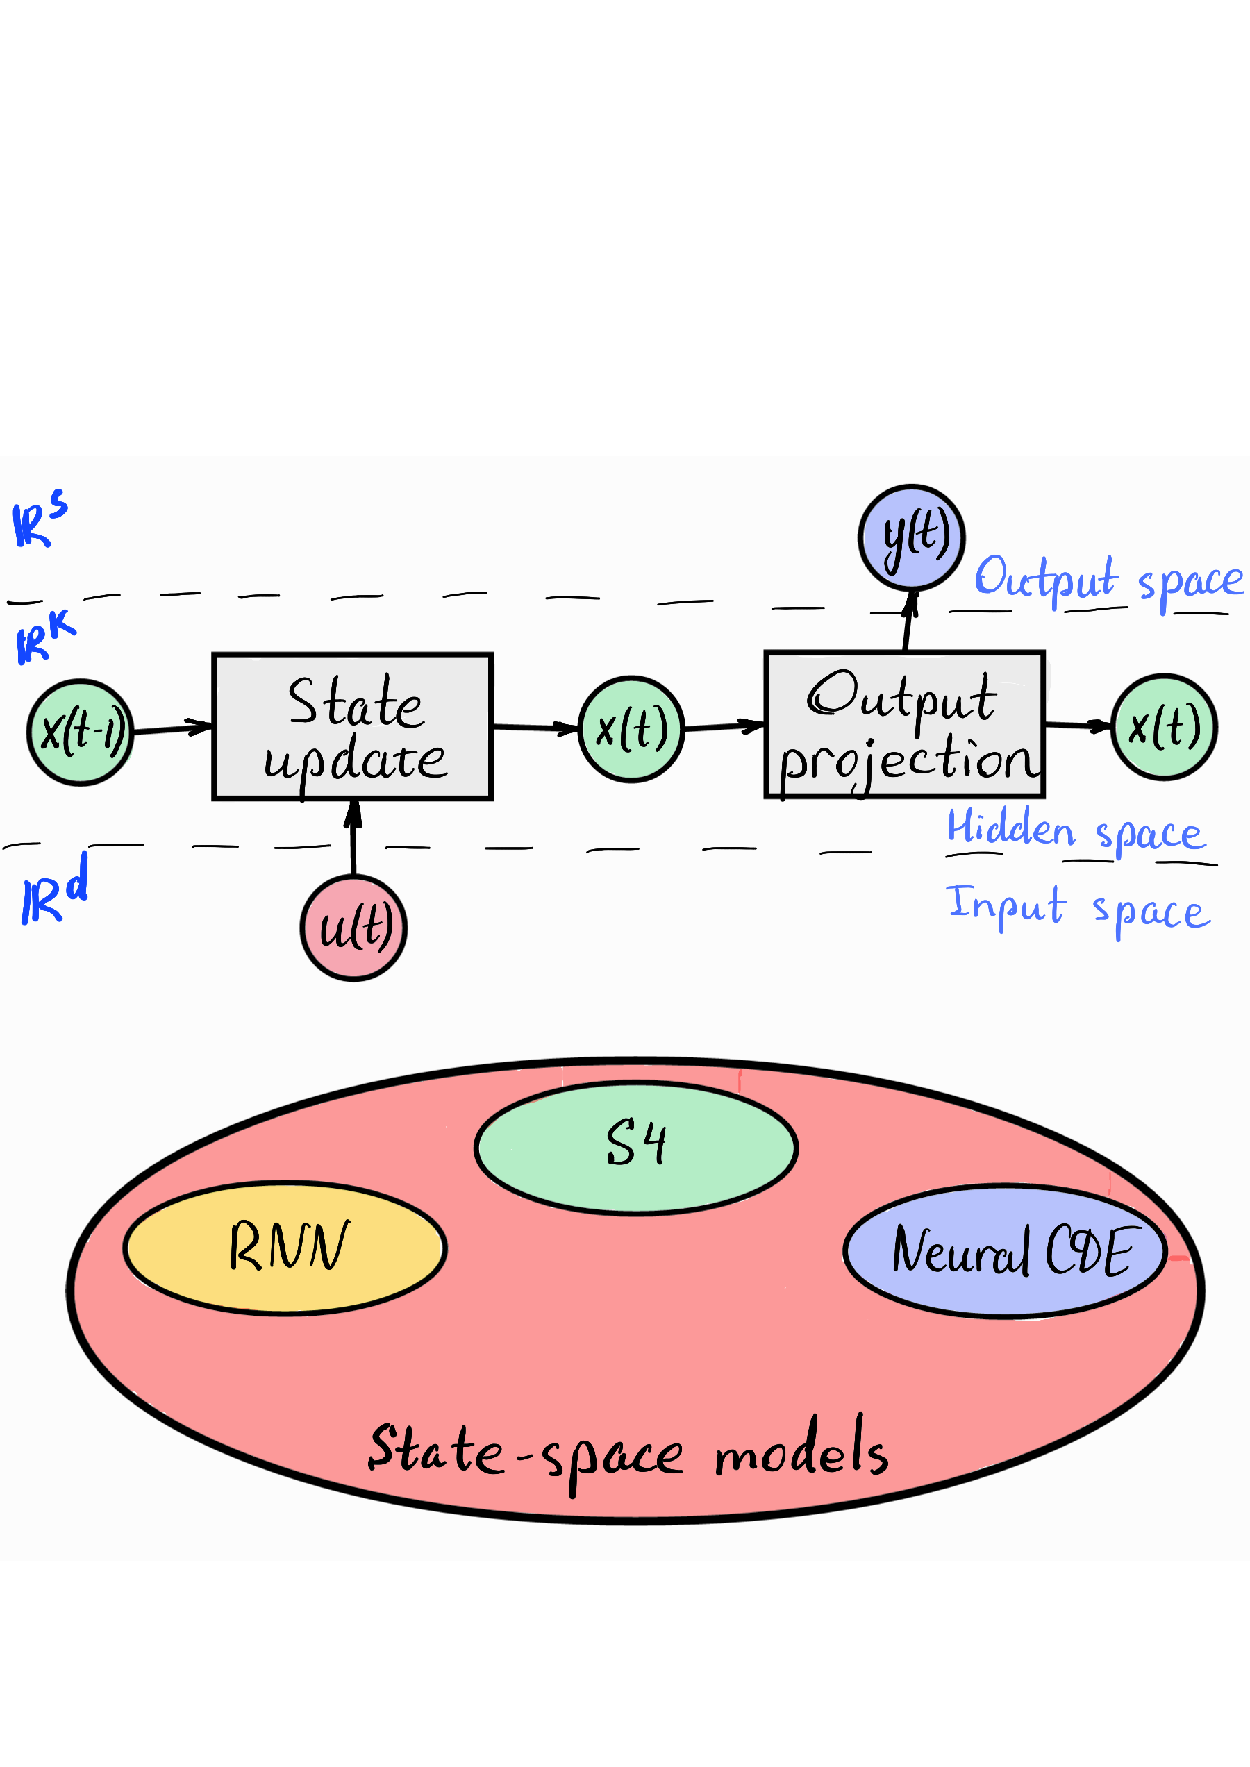
\includegraphics[width=0.45\textwidth]{3rd-slide-2.pdf}
		
		\begin{gather*}
			\text{Непрерывная модель пр-ва состояний} \\
			x'(t) = Ax(t) + Bu(t) \\
			y(t) = Cx(t) + \stkout{Du(t)} \\
			\text{Дискретная модель пр-ва состояний} \\
			x_k = Ax_{k-1} + Bu_k \\
			y_k = Cx_k + \stkout{Du_k}
		\end{gather*}
	
		\begin{table}[bhtp]
			\begin{tabular}{|l|l|l|}
				\hline
				\multicolumn{1}{|c|}{SSM} & \multicolumn{1}{c|}{CNN} & \multicolumn{1}{c|}{Transformer} \\ \hline
				LSTM & EEGNet & GPT \\
				??? & HTNet & Wav2Vec \\
				\hline
			\end{tabular}
		\end{table}
	
	\end{multicols}
\end{frame}

%--------------------------------------------------------------------------------------------------------

\begin{frame}{Постановка задачи классификации сигнала ЭКоГ}
	$\bX \in \dR^{M \times N \times T}$ ~--- $M$ измерений ЭКоГ, где $N$ ~--- число электродов, $T$ ~--- число элементов временного ряда
	
	$Y \in \{ 0, 1\}^M$ ~--- целевая переменная
	
	Критерий качества ~--- бинарная кросс-энтропия  
	
	$$ L(\bw) = -\dfrac{1}{M} \sum\limits_{m=1}^M y_m \log(f(\bw, \bx)) + (1 - y_m) \log(1 - f(\bw, \bx))$$
	
	Оптимизационная задача: $\hat{\bw} = \underset{\bw}{\arg \max} L(\bw)$
\end{frame}

%---------------------------------------------------------------------------------------------------------
\begin{frame}{Рекуррентные нейронные сети (RNN)}
	\begin{multicols}{2}
		\begin{figure}
			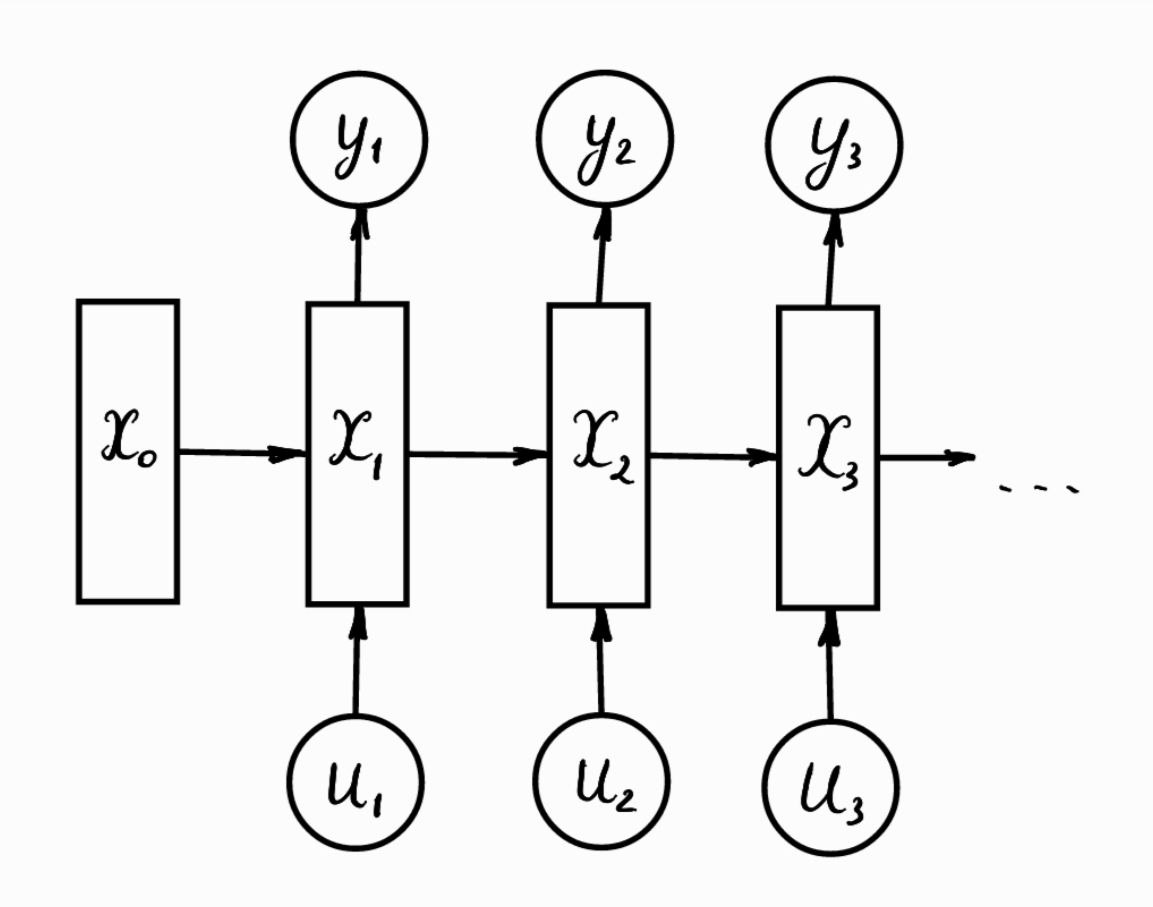
\includegraphics[width=0.5\textwidth]{rnn.jpg}
		\end{figure}
		
		\begin{equation*}
			\mbox{\Large\(
				\begin{aligned}
					\bx_t &= \sigma_x(W_x \bx_{t-1} + W_u \bu_t) \\
					\by_t &= \sigma_y(W_y \bx_t),
				\end{aligned}
			\)}
		\end{equation*}
		$\text{где } \bu_i \in \dR^d, \; \bx_i \in \dR^K \; \by_i \in \dR^s$  
		
		$\sigma: \dR^K \rightarrow \dR^K$ ~--- функция активации  
		
		$W_x \in \dR^{K \times K}, W_u \in \dR^{s \times K}, W_y \in \dR^{K \times d}$ ~--- матрицы весов
	\end{multicols}
	\bigskip
	\footnotetext[1]{\textit{Rumelhart, David E and Hinton, Geoffrey E and Williams, Ronald J} Learning internal representations by error propagation //California Univ San Diego La Jolla Inst for Cognitive Science – 1985}
\end{frame}
%----------------------------------------------------------------------------------------------------------
\begin{frame}{Свойства модели RNN}
	Количество параметров = $K^2 + Ks + Kd = O(KM)$
	
	Время прямого прохода = $O(KML)$, где $M = \max(d, K, s)$
	
	\begin{table}[bhtp]
		\begin{tabularx}{0.95\textwidth}{|X|X|}
			\hline
			Преимущества & Недостатки \\ \hline
				есть реализация во всех фреймворках глубокого обучения & не работают с данными, содержащими пропуски и/или разной частотой сэмплирования \\ относительно быстрое обучение и предсказание модели & \\ \hline
		\end{tabularx}
	\end{table}
\end{frame}

%----------------------------------------------------------------------------------------------------------
\begin{frame}{Нейронные контролируемые дифференциальные уравнения (NCDE/Neural CDE)}
	\begin{multicols}{2}
		\begin{figure}
			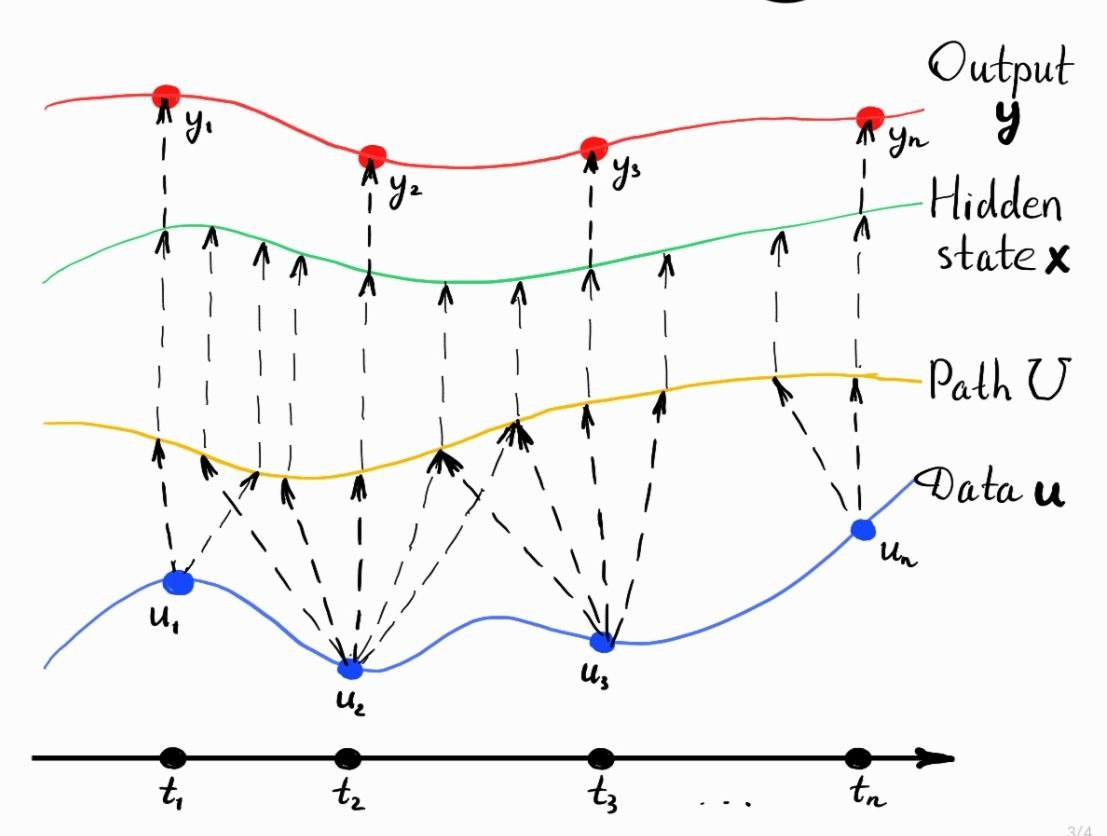
\includegraphics[width=0.5\textwidth]{neural-cde-path.jpg}
		\end{figure}
	
		\begin{equation*}
			\begin{cases}
				\bx(t_1) = \zeta(\bu_1, t_1) \\
				\bx(t) = \bx(t_1) + \int_{t_1}^t \bff(\bx(\tau))dU(\tau) \\
				\by_i = g(\bx(t_i))
			\end{cases}
		\end{equation*}
		$\text{где } \bu_i \in \dR^d, \; \by_i \in \dR^s $
		
		$\bx: [t_1, t_n] \rightarrow \dR^K$ ~--- функция скрытого состояния
		
		$U: [t_1, t_n] \rightarrow \dR^{d+1}$ ~--- кубический сплайн 
		
		$\zeta: \dR^{d+1} \rightarrow \dR^K$ ~--- проектор в скрытое пространство
		
		$f: \dR^K \rightarrow \dR^{K \times (d+1)}$ ~--- динамика скрытого состояния
		
		$g: \dR^K \rightarrow \dR^s$ ~--- линейное отображение
	\end{multicols}
\end{frame}

%----------------------------------------------------------------------------------------------------------
\begin{frame}{Свойства модели NCDE}
	Количество параметров = $O(K^2d + Ks)$
	
	Время прямого прохода = $O(K^2dL)$
	
	\begin{table}[bhtp]
		\begin{tabularx}{0.95\textwidth}{|X|X|}
			\hline
			Преимущества & Недостатки \\ \hline
			большая гибкость в настройке модели: выбор архитектуры функции $\bff(\bx)$ и пути $U(t)$ & в десятки раз медленнее, чем RNN \\ 
			работает с данными, в которых содержатся пропуски и которые имеют разную частоту сэмплирования &  на текущий момент не существует эффективной реализации \\
			 & долгая настройка модели \\ & \\
			 & нестабильное обучение при больших $K$, при использовании солверов с адаптивным шагом и функции активации ReLU \\
			\hline
		\end{tabularx}
	\end{table}
	
	\bigskip
	\footnotetext[1]{\textit{Kidger P. et al.} Neural controlled differential equations for irregular time series //Advances in Neural Information Processing Systems. – 2020. – Т. 33. – С. 6696-6707}
\end{frame}

%----------------------------------------------------------------------------------------------------------
\begin{frame}{Модели структурированного пространства состояний (S4)}
	\begin{figure}[bhtp]
		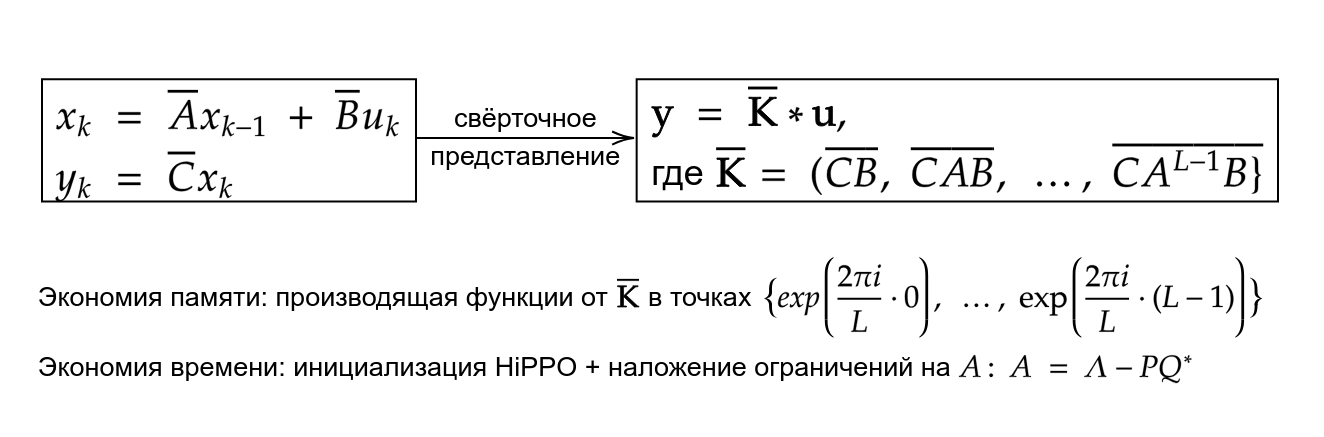
\includegraphics[width=\textwidth]{s4-schema.png}
		\label{fig:s4}
	\end{figure}
\end{frame}

\begin{frame}{Свойства модели S4}
	Количество параметров = $Kd + Ks$
	
	Время прямого прохода = $O(KML)$
	
	\begin{table}[bhtp]
		\begin{tabularx}{0.95\textwidth}{|X|X|}
			\hline
			Преимущества & Недостатки \\ \hline
			хорошо работает с данными, содержащими долговременные зависимости & в несколько раз медленнее, чем RNN \\ 
			существует эффективная реализация & не работают с данными, содержащими пропуски и/или разной частотой сэмплирования \\
			\hline
		\end{tabularx}
	\end{table}
	
	\bigskip
	\footnotetext[1]{\textit{Gu, Albert, Karan Goel, and Christopher Ré} Efficiently modeling long sequences with structured state spaces //arXiv preprint arXiv:2111.00396. – 2021}
\end{frame}
%----------------------------------------------------------------------------------------------------------
\begin{frame}{Итоговое сравнение моделей}
	$L$ ~--- длина последовательности
	
	$d$ ~--- размерность исходного пространства
	
	$K$ ~--- размерность скрытого пространства (в случае с CNN ~--- размер ядра)
	
	$s$ ~--- размерность целевого пространства
	
	$N$ ~--- количество датчиков ЭКоГ
	
	$M = \max(d, K, s)$  
	
	\begin{table}[bhtp]
		\centering
		\caption{Сравнение моделей по числу обучаемых параметров, времени прямого прохода, наличию эффективной реализации, возможности работы с пропусками и хранения всей истории}
		\begin{tabularx}{0.99\textwidth}{c|c|c|X|X|X|}
			\cline{2-6}
			\multicolumn{1}{l|}{}             & Parameters & Forward & Fast impl. & Cont. time & Unb. context \\ \hline
			\multicolumn{1}{|c|}{RNN}         & $O(KM)$ & $O(KML)$ & $+$ & $-$ & $+$ \\ \hline
			\multicolumn{1}{|c|}{NCDE}  & $O(K^2d + Ks)$ & $O(K^2dL)$ & $-$ & $+$ & $+$ \\ \hline
			\multicolumn{1}{|c|}{S4}          & $O(Kd + Ks)$ & $O(KML)$ & $+$ & $-$ & $+$ \\ \hline
			\multicolumn{1}{|c|}{Transformer} & $O(K^2d + Ks)$ & $O(LK \cdot (L+s))$ & $+$ & $-$ & $+$ \\ \hline
			\multicolumn{1}{|c|}{CNN} & $O(K^2)$ & $O(K^2(L-K)(N-K))$ & $+$ & $-$ & $-$ \\ \hline
		\end{tabularx}
	\end{table}
\end{frame}
%----------------------------------------------------------------------------------------------------------
\begin{frame}{Вычислительный эксперимент на данных ЭКоГ}
	\begin{varblock}{Цель}
		 На примере задачи классификации сигналов ЭКоГ сравнить работу различных моделей пространства состояний
	\end{varblock}
	
	\begin{multicols}{2}
		\begin{figure}
			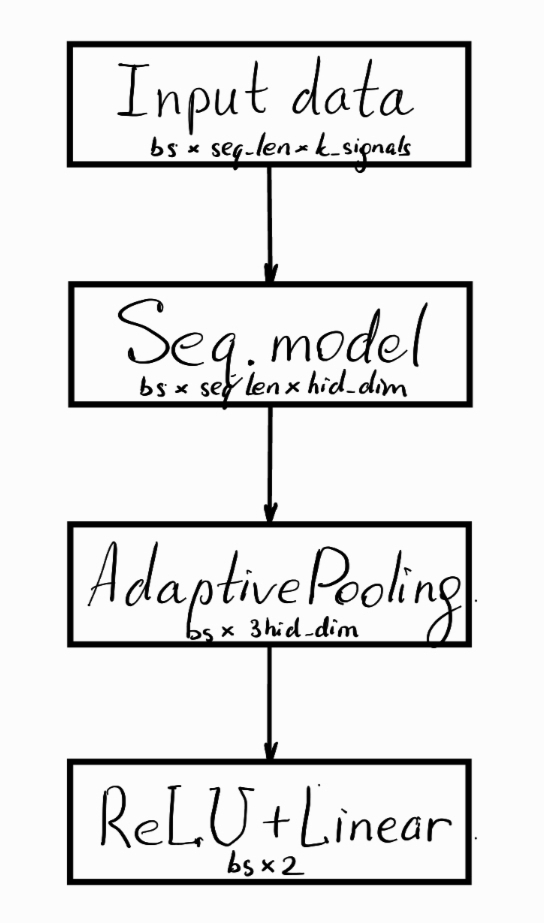
\includegraphics[height=0.65\textheight]{seq-model.jpg}
		\end{figure}
	
		\begin{varblock}[6cm]{Данные}
			ЭКоГ-записи были получены от 12 участников
			в ходе клинического мониторинга эпилепсии. Эти записи длятся 7 $\pm$ 2 дня на каждого участника. ЭКоГ сигнал измерялся 126 каналами с частотой 250 Гц. Один сэмпл соответствует 2 секундам записи сигнала, во время которых участник двигал или не двигал рукой.
		\end{varblock}
	
		Train/Val/Test = 7/4/1
		
		Количество разбиений = 20
		
	\end{multicols}
\end{frame}

%----------------------------------------------------------------------------------------------------------
\begin{frame}{Анализ ошибки моделей декодирования}
	\begin{figure}
		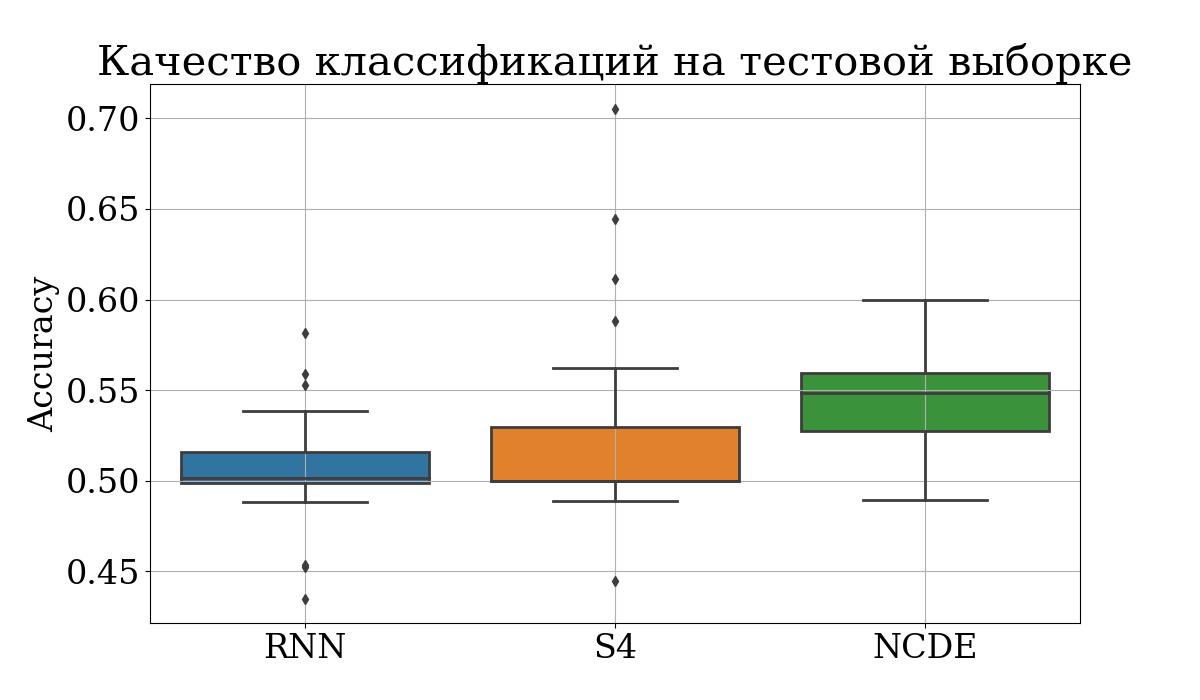
\includegraphics[width=0.5\textwidth]{rnn-s4-ncde.png}
	\end{figure}

	\begin{table}
		\begin{tabular}{c|l|l|l|}
			\cline{2-4}
			\multicolumn{1}{l|}{}  & Parameters & Time per epoch (sec) & Accuracy \\ \hline
			\multicolumn{1}{|c|}{RNN} & 34.2k & 5.86 & 0.506 $\pm$ 0.027 \\ \hline
			\multicolumn{1}{|c|}{S4} & 33.3k & 10.07 & 0.521 $\pm$ 0.049 \\ \hline
			\multicolumn{1}{|c|}{Neural CDE} & 31.5k & 37.23 & 0.546 $\pm$ 0.026 \\ \hline
		\end{tabular}
	\end{table}
\end{frame}

%----------------------------------------------------------------------------------------------------------
\begin{frame}{Выносится на защиту}
	\begin{enumerate}
		\item Рассмотрено применение моделей пространства состояний в задаче классификации сигналов ЭКоГ
		
		\item Изучены свойства следующих моделей пространства состояний: RNN, NCDE, S4
		
		\item Предоставлена рекомендация по выбору моделей пространства состояния
		
		\item Продемонстрировано, что модель Neural CDE имеет лучшее качество на тестовой выборке по сравнению с другими моделями, однако её время обучения сильно превышает время обучения других моделей
	\end{enumerate}
\end{frame}

\end{document} 